\hspace{24pt}

In Section~\ref{sec:result}, we have seen that the best performance of the zh-ja NMT system can be achieved by utilizing Jieba \& Janome as the tokenization method and the joint embedding as an additional feature in the Transformer model. Based on the promising performance of the models, we will further examine the translation results produced by the best model and try to explain the reasons for its better translation in Section~\ref{sec:case_study}. In addition, we will compare the joint embedding with the semantic embedding in Section~\ref{sec:analysis} to further analyze the advantages that the joint embedding provides over traditional embedding.

\section{Case Study} \label{sec:case_study}

We compare the translation results using joint embedding with those using semantic embedding. The results show that the uses of the joint embedding are much better than that of semantic embedding in four aspects.

\vspace{0.4cm}
\begin{table}[h]
    \centering
    \begin{CJK}{UTF8}{gbsn}
        \begin{tabularx}{\textwidth}{p{1.2cm}b}\toprule
            Source & 使用有机溶剂的溶剂提取法作为物质的分离手段被广泛利用。 \\
        \end{tabularx}
    \end{CJK}

    \begin{CJK}{UTF8}{long}
        \begin{tabularx}{\textwidth}{p{1.2cm}b}
            Target & 有機溶媒を用いた溶媒抽出法は物質の分離手段として広く利用されている。 \\
            Semantic & 有機溶媒を用いた溶媒抽出法は物質の分離手段として広く\underline{用いされ}ている。 \\
            Joint & 有機溶媒を用いた溶媒抽出法は物質の分離手段として広く\underline{利用され}ている。 \\\midrule
        \end{tabularx}
    \end{CJK}

    \begin{CJK}{UTF8}{gbsn}
        \begin{tabularx}{\textwidth}{p{1.2cm}b}
            Source & 在本章中,将分布式组件间进行通信的中间件与Dragon进行比较。 \\
        \end{tabularx}
    \end{CJK}

    \begin{CJK}{UTF8}{long}
        \begin{tabularx}{\textwidth}{p{1.2cm}b}
            Target & 本章では,分散コンポーネント間通信を行うミドルウェアとDragonを比較する. \\
            Semantic & 本章では,\underline{分散コンポーネント間}でを行うミドルウェアとDragonを比較する. \\
            Joint & 本章では,\underline{分散コンポーネント間通信}を行うミドルウェアとDragonを比較する. \\\midrule
        \end{tabularx}
    \end{CJK}

    \begin{CJK}{UTF8}{gbsn}
        \begin{tabularx}{\textwidth}{p{1.2cm}b}
            Source & LearnAR从背景知识B和观测结果O中获得行动规则的集合γ的集合H。 \\
        \end{tabularx}
    \end{CJK}

    \begin{CJK}{UTF8}{long}
        \begin{tabularx}{\textwidth}{p{1.2cm}b}
            Target & LearnARは,背景知識Bと観測結果Oより行動規則の集合γ\underline{の集合を}獲得する. \\
            Semantic & LearnARは\underline{背景背景知識}Bと観測結果Oから\underline{行動ルール}の集合γの集合H獲得する. \\
            Joint & LearnARは,\underline{背景知識}Bと観測結果Oから\underline{行動規則}の集合γ\underline{の集合H}獲得する. \\\midrule
        \end{tabularx}
    \end{CJK}

    \caption{Case Study - Preservation of correct words}
    \label{tab:case_study1}
\end{table}

\begin{CJK}{UTF8}{long}
    Table~\ref{tab:case_study1} compares the results of the two translations in terms of their ability to preserve correct words. In the first result, ``利用され'' (be used) is correctly translated by the joint embedding, while ``用いされ'' is the wrong translation, which is usually expressed by using ``用いられ''. In the second result, ``分散コンポーネント間通信'' (communication between distributed components) is correctly translated by the joint embedding, and the semantic embedding omits ``通信'' (communication). In the third result, the joint embedding produced the best translation. It successfully translated the symbol $H$ that was not present in the target sentence and made the whole sentence more fluent than the result from the semantic embedding.
\end{CJK}

\vspace{0.4cm}
\begin{table}[h]
    \centering

    \begin{CJK}{UTF8}{gbsn}
        \begin{tabularx}{\textwidth}{p{1.2cm}b}\toprule
            Source & 构成这些乐曲时在可能范围里保证变化丰富。 \\
        \end{tabularx}
    \end{CJK}

    \begin{CJK}{UTF8}{long}
        \begin{tabularx}{\textwidth}{p{1.2cm}b}
            Target & これらの楽曲は,可能な範囲でバリエーションが豊かになるように構成されている. \\
            Semantic & これらの楽曲を,豊かな範囲で\underline{変化}が豊かになる.にしされている. \\
            Joint & これらの楽曲を,可能な範囲で\underline{バリエーション}が豊かになるように構成されている. \\\midrule
        \end{tabularx}
    \end{CJK}

    \begin{CJK}{UTF8}{gbsn}
        \begin{tabularx}{\textwidth}{p{1.2cm}b}
            Source & 铝焊接烟气的特性 \\
        \end{tabularx}
    \end{CJK}

    \begin{CJK}{UTF8}{long}
        \begin{tabularx}{\textwidth}{p{1.2cm}b}
            Target & アルミニウム溶接ヒュームの物性 \\
            Semantic & アルミニウム溶接\underline{煙}の特性 \\
            Joint & アルミニウム溶接\underline{ヒューム}の特性 \\\midrule
        \end{tabularx}
    \end{CJK}
    \caption{Case Study - Preservation of Katakana}
    \label{tab:case_study2}
\end{table}

\begin{CJK}{UTF8}{long}
    Table~\ref{tab:case_study2} demonstrates the ability of joint embedding to preserve Katakana. Katakana is the Japanese word exactly translated from the foreign language, and it can represent foreign languages more precisely. In the first result, ``バリエーション'' fully expresses the meaning of ``variation'', while ``変化'' can refer to other meanings such as ``change, alteration, and inflection''. In the second result, ``ヒューム'' is equal to ``fume'', while ``煙'' stands for ``smoke'', which is far from the meaning of ``fume''. The reason for the preservation of Katakana possibly because it is composed of phonetic characters. Consequently, the joint embedding emphasizes the phonetic information, which allows Katakana to be better preserved by the model.
\end{CJK}

\vspace{0.4cm}
\begin{table}[h]
    \centering

    \begin{CJK}{UTF8}{gbsn}
        \begin{tabularx}{\textwidth}{p{1.2cm}b}\toprule
            Source & RMCPRGIGCenter和RMCPRGIGTransceiver使用C语言安装,在二者间的通信中和RemoteGIG同样使用TCP/IP上的RMCP。 \\
        \end{tabularx}
    \end{CJK}

    \begin{CJK}{UTF8}{long}
        \begin{tabularx}{\textwidth}{p{1.2cm}b}
            Target & RMCPRGIGCenterとRMCPRGIGTransceiverはC言語で実装し,両者間の通信にはRemoteGIGと同様にTCP/IP上のRMCPを用いた. \\
            Semantic & RMCPRGIGCenterと\underline{RMCPRGIGTranscei}はC言語を実装し,両者間通信通信で\underline{TCPTCP}と同様にTCP/IPででRMCPを用いるて. \\
            Joint & RMCPRGIGCenterと\underline{RMCPRGIGTransceiver}をC言語を実装し,両者間の通信においては\underline{RemoteGIG}と同様にTCP/IP上でRMCPを用いた. \\\midrule
        \end{tabularx}
    \end{CJK}

    \begin{CJK}{UTF8}{gbsn}
        \begin{tabularx}{\textwidth}{p{1.2cm}b}
            Source & 另一方面,GUIServer和GUIClient是用Java语言进行安装。 \\
        \end{tabularx}
    \end{CJK}

    \begin{CJK}{UTF8}{long}
        \begin{tabularx}{\textwidth}{p{1.2cm}b}
            Target & 一方,GUIServerとGUIClientはJava言語で実装した. \\
            Semantic & 一方,\underline{GUISverver}や\underline{GUIIClient}はJava言語で実装した. \\
            Joint & 一方,\underline{GUIServer}と\underline{GUIClient}はJava言語で実装した. \\\midrule
        \end{tabularx}
    \end{CJK}

    \caption{Case Study - Preservation of English words}
    \label{tab:case_study3}
\end{table}

\begin{CJK}{UTF8}{long}
    Table~\ref{tab:case_study3} demonstrates the ability of joint embedding to cope with English text. When English words are present, semantic embedding often produces incorrect translations. It will lose English words, generate the wrong English words and grammar. On the contrary, joint embedding can generate the correct English words and have the correct grammar.
\end{CJK}

\begin{table}[h]
    \centering

    \begin{CJK}{UTF8}{gbsn}
        \begin{tabularx}{\textwidth}{p{1.2cm}b}\toprule
            Source & 微小粒子测量装置的比较试验 \\
        \end{tabularx}
    \end{CJK}

    \begin{CJK}{UTF8}{long}
        \begin{tabularx}{\textwidth}{p{1.2cm}b}
            Target & 微小粒子測定装置の比較試験 \\
            Semantic & 微小粒子\underline{計測}装置の比較\underline{実験} \\
            Joint & 微小粒子\underline{測定}装置の比較\underline{試験} \\\midrule
        \end{tabularx}
    \end{CJK}

    \begin{CJK}{UTF8}{gbsn}
        \begin{tabularx}{\textwidth}{p{1.2cm}b}
            Source & 胃运动机能和NERD的病状的关连性的相关讨论 \\
        \end{tabularx}
    \end{CJK}

    \begin{CJK}{UTF8}{long}
        \begin{tabularx}{\textwidth}{p{1.2cm}b}
            Target & 胃運動機能とNERDの病態との関連性に関する検討 \\
            Semantic & 胃運動機能とNERDの病態\underline{の}の関連性に関する\underline{議論} \\
            Joint & 胃運動機能とNERDの病態\underline{と}の関連性に関する\underline{検討} \\\midrule
        \end{tabularx}
    \end{CJK}

    \begin{CJK}{UTF8}{gbsn}
        \begin{tabularx}{\textwidth}{p{1.2cm}b}
            Source & 此外,用100对属性数进行了均等化。 \\
        \end{tabularx}
    \end{CJK}

    \begin{CJK}{UTF8}{long}
        \begin{tabularx}{\textwidth}{p{1.2cm}b}
            Target & また,属性数を100で均一化した. \\
            Semantic & また,属性数を100で\underline{均等化}した. \\
            Joint & また,属性数を100で\underline{均一化}した. \\\midrule
        \end{tabularx}
    \end{CJK}

    \caption{Case Study - Improvements of word selection}
    \label{tab:case_study4}
\end{table}

\begin{CJK}{UTF8}{long}
    Table~\ref{tab:case_study4} shows that joint embedding will select more precise words for translation. In the first result, ``測定装置'' is more commonly used to indicate ``measuring instruments'', while ``計測'' is more often used independently to indicate ``instrumentation'', that is, using instruments to measure. In addition, joint embedding also correctly translates ``试验'' (test) from Chinese to ``試驗'' (test) rather than ``実験'' (experiment). In the second result, it is better to use ``検討'' (study, examination) than ``議論'' (debate, argument) for the study of disease. In the third result, it is also better to use ``均一化'' (regularization) than ``均等化'' (equalization) in the context. It is possible that the semantic embedding is more influenced by the Chinese to produce the identical text as the Chinese.
\end{CJK}

\section{Embedding Analysis} \label{sec:analysis}

We applied four analysis methods to compare joint embedding and semantic embedding. In all four analyses, joint embedding preserves the properties that semantic embedding should have and even outperforms semantic embedding.

\subsection{Analogical Reasoning} \label{sec:analysis_analogy}

The joint embedding can reason out the correct answer in the analogical reasoning task as the semantic embedding, which is to solve for $a-a*+b$. We found that the answers obtained from joint embedding received higher confidence values on average in both Chinese (Table~\ref{tab:analysis_analogy1}) and Japanese (Table~\ref{tab:analysis_analogy2}). 

\begin{table}[h]
    \centering
    \begin{CJK}{UTF8}{gbsn}
        \begin{tabularx}{\textwidth}{lllbb}
            \toprule
            \multicolumn{3}{c}{Input} & \multicolumn{2}{c}{Output ($b*$)} \\
            \cmidrule(lr){1-3} \cmidrule(lr){4-5} $a$ & $a*$ & $b$ & Semantic & Joint \\\midrule
            \vspace{0.2cm} 东京 (Tokyo) & 日本 (Japan) & 北京 (Beijing) & 中国 (China) \newline ($p=0.492$) & 中国 (China) \newline ($\bm{p=0.531}$) \\
            \vspace{0.2cm} 长期 (long-term) & 三年 (3 years) & 短期 (short-term) & 一年 (1 year) \newline ($p=0.379$) & 两周 (2 weeks) \newline ($\bm{p=0.387}$) \\
            进口 (import) & 买入 (buy) & 出口 (export) & 卖出 (sell) \newline ($p=0.364$) & 卖出 (sell) \newline ($\bm{p=0.442}$)\\\bottomrule
        \end{tabularx}
    \end{CJK}
    \caption{Analogical Reasoning in Chinese}
    \label{tab:analysis_analogy1}
\end{table}

\begin{table}[h]
    \centering
    \begin{CJK}{UTF8}{long}
        \begin{tabularx}{\textwidth}{lllbb}
            \toprule
            \multicolumn{3}{c}{Input} & \multicolumn{2}{c}{Output ($b*$)} \\
            \cmidrule(lr){1-3} \cmidrule(lr){4-5} $a$ & $a*$ & $b$ & Semantic & Joint \\\midrule
            \vspace{0.2cm} 男性(male) & 女性 (female) & 父親 (father) & 母親 (mother) \newline ($p=0.487$) & 母親 (mother) \newline ($\bm{p=0.508}$) \\
            \vspace{0.2cm} 長期 (long-term) & 年 (year) & 短期 (short-term) & 月 (month) \newline ($p=0.550$) & 月 (month) \newline ($\bm{p=0.570}$) \\
            左右(left-right) & 前後 (front-rear) & 水平 (horizontal) & 垂直 (vertical) \newline ($\bm{p=0.432}$) & 垂直 (vertical) \newline ($p=0.402$) \\\bottomrule
        \end{tabularx}
    \end{CJK}
    \caption{Analogical Reasoning in Japanese}
    \label{tab:analysis_analogy2}
\end{table}

\subsection{Outlier Detection} \label{sec:analysis_outlier}

\begin{CJK}{UTF8}{gbsn}    
    Joint embedding can answer outlier detection problems as well as semantic embedding, and sometimes gives better answers. For example, in the second case of Table~\ref{tab:analysis_outlier1}, the joint embedding answers correctly, while semantic embedding answers incorrectly.
\end{CJK}

\begin{table}[h]
    \centering
    \begin{CJK}{UTF8}{gbsn}
        \begin{tabularx}{\textwidth}{bll}
            \toprule
            \multirow{2.5}{*}{Word Cluster} & \multicolumn{2}{c}{Outlier (Output)} \\
            \cmidrule(lr){2-3} {} & Semantic & Joint \\\midrule

            鸟 (birds), 狗 (dogs), 猫 (cats), 花 (flowers) & \vspace{0.25cm} 花 (flowers) & 花 (flowers) \\

            可行(feasible), 不行 (not OK), 行 (OK), 可以 (can) & \vspace{0.25cm} 可以 (can) & 不行 (not OK) \\

            广岛 (Hiroshima, Japan), 名古屋 (Nogoya, Japan), 爱知(Aichi, Japan), 上海 (Shanghai, China) & 上海 (Shanghai, China) & 上海 (Shanghai, China)\\\bottomrule
        \end{tabularx}
    \end{CJK}
    \caption{Outlier Detection in Chinese}
    \label{tab:analysis_outlier1}
\end{table}

\begin{table}[h]
    \centering
    \begin{CJK}{UTF8}{long}
        \begin{tabularx}{\textwidth}{bll}
            \toprule
            \multirow{2.5}{*}{Word Cluster} & \multicolumn{2}{c}{Outlier (Output)} \\
            \cmidrule(lr){2-3} {} & Semantic & Joint \\\midrule
            生み (birth), 創造 (creation), 作る (making), 破壊 (destruction) & \vspace{0.25cm} 破壊 (destruction) & 破壊 (destruction) \\
            普通 (normal), 一般 (general), 通常 (commonly), 異常 (abnormal) & \vspace{0.25cm} 異常 (abnormal) & 異常 (abnormal) \\
            平成 (Heisei era), 昭和 (Showa era), 大正 (Taisho era), 明治 (Meiji era), 京都 (Kyoto prefecture) & 京都 (Kyoto prefecture) & 京都 (Kyoto prefecture) \\\bottomrule
        \end{tabularx}
    \end{CJK}
    \caption{Outlier Detection in Japanese}
    \label{tab:analysis_outlier2}
\end{table}

\vspace{0.4cm}
\begin{figure}[h!]
    \begin{CJK}{UTF8}{gbsn}
    \centering
    \begin{subfigure}[b]{0.49\textwidth}
        \centering
        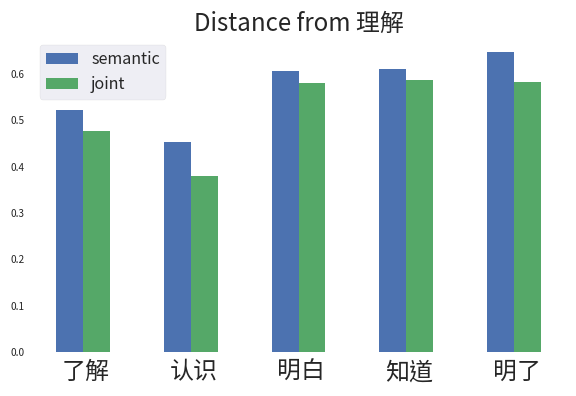
\includegraphics[width=\textwidth]{../images/similarity_zh1.png}
        \caption{Similarity distances between ``理解'' (comprehend) and its synonyms are decreasing in the joint embedding}
        \label{fig:similarity_zh1}
    \end{subfigure}
    \hfill
    \begin{subfigure}[b]{0.49\textwidth}
        \centering
        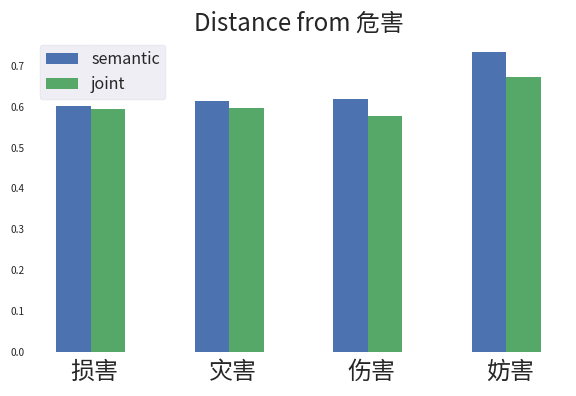
\includegraphics[width=\textwidth]{../images/similarity_zh2.png}
        \caption{Similarity distances between ``危害'' (jeopardize) and its synonyms are decreasing in the joint embedding}
        \label{fig:similarity_zh2}
    \end{subfigure}
    \begin{subfigure}[b]{0.49\textwidth}
        \centering
        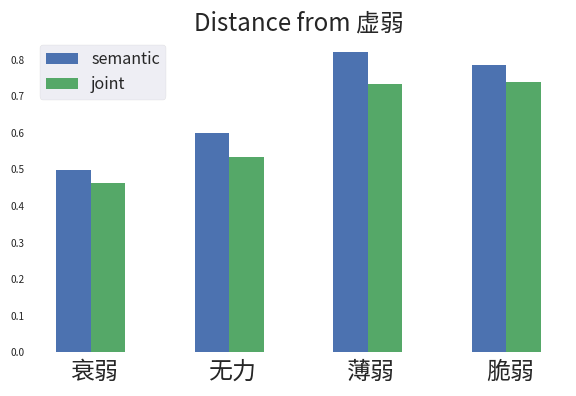
\includegraphics[width=\textwidth]{../images/similarity_zh3.png}
        \caption{Similarity distances between ``虛弱'' (weak) and its synonyms are decreasing in the joint embedding}
        \label{fig:similarity_zh3}
    \end{subfigure}
    \begin{subfigure}[b]{0.49\textwidth}
        \centering
        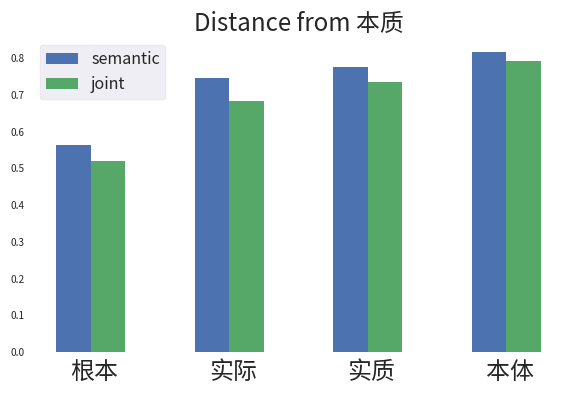
\includegraphics[width=\textwidth]{../images/similarity_zh4.png}
        \caption{Similarity distances between ``本质'' (essence) and its synonyms are decreasing in the joint embedding}
        \label{fig:similarity_zh4}
    \end{subfigure}
    \caption{The Similarity Distances Between Synonyms in Chinese}
	\label{fig:similarity_zh}
\end{CJK}
\end{figure}

\subsection{Word Similarity} \label{sec:analysis_similarity}
\begin{CJK}{UTF8}{gbsn}
    The similarity distance between synonyms is not only preserved but also shortened. This finding indicates the joint embedding not only protects but also enhances the semantics by adding phonetic information. Figure~\ref{fig:similarity_zh} shows that the similarity distances of Chinese synonyms are all shortened in the joint embedding. For example, Figure~\ref{fig:similarity_zh1} shows that the distance between ``了解 (understand), 认识 (recognize), 明白 (realize), 知道 (know), 明了 (clearly understand)'' and ``理解 (comprehend)'' are decreasing in the joint embedding.

    % ``了解 (understand), 认识 (recognize), 明白 (realize), 知道 (know), 明了 (clearly understand)'', ``理解 (comprehend)'' 
    
    % ``损害 (harm), 灾害 (calamity), 伤害 (injure), 妨害 (impair)'', ``危害 (jeopardize)''
    
    % ``衰弱 (feeble), 无力 (powerless), 薄弱 (frail), 脆弱 (fragile)', ``虚弱 (weak)''. 
    
    % ``根本 (fundamental), 实际 (reality), 实质 (substance), 本体 (ontology)'', ``本质 (essence)''.
\end{CJK}

\begin{CJK}{UTF8}{long}
    Similarly, the similarity distances of Japanese synonyms are also shortened with the use of joint embedding. Especially in Japanese, sometimes Hiragana and Kanji are used interchangeably. For example, in Figure~\ref{fig:similarity_ja4}, ``また'' and ``又 (また)'' have the same spelling and meaning (i.e., ``again''). The joint embedding can find the relationship between them and reduce their distance significantly.
\end{CJK}

\vspace{0.4cm}
\begin{CJK}{UTF8}{long}
    \begin{figure}[h]
        \centering
        \begin{subfigure}[b]{0.49\textwidth}
            \centering
            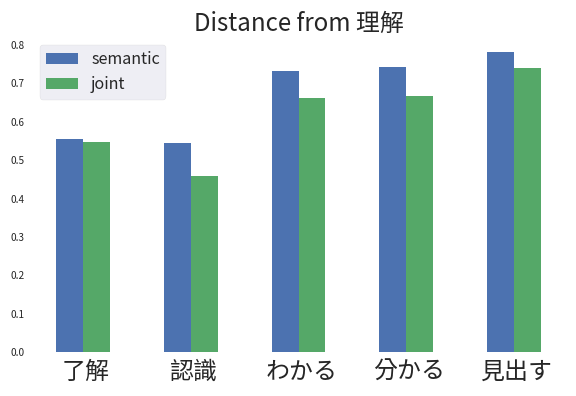
\includegraphics[width=\textwidth]{../images/similarity_ja1.png}
            \caption{Similarity distances between ``理解'' (comprehend) and its synonyms are decreasing in the joint embedding}
            \label{fig:similarity_ja1}
        \end{subfigure}
        \hfill
        \begin{subfigure}[b]{0.49\textwidth}
            \centering
            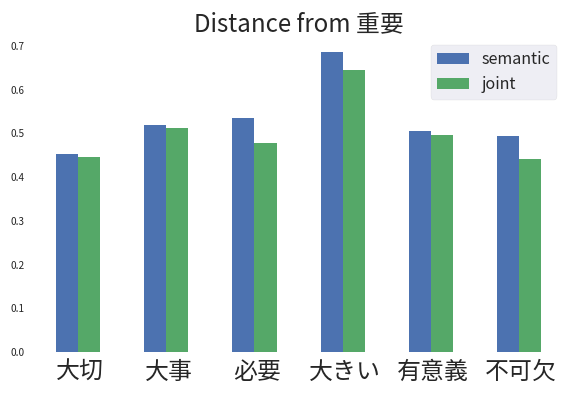
\includegraphics[width=\textwidth]{../images/similarity_ja2.png}
            \caption{Similarity distances between ``重要''' (important) and its synonyms are decreasing in the joint embedding}
            \label{fig:similarity_ja2}
        \end{subfigure}
        \begin{subfigure}[b]{0.49\textwidth}
            \centering
            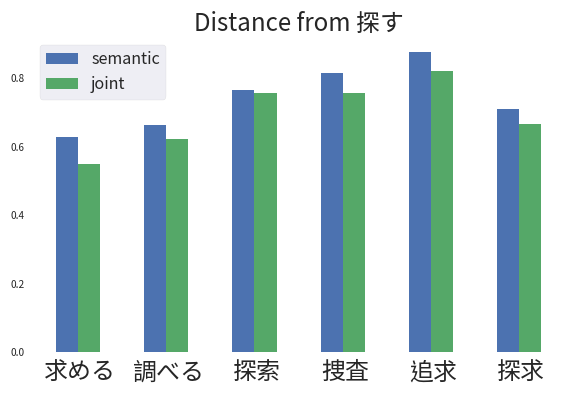
\includegraphics[width=\textwidth]{../images/similarity_ja3.png}
            \caption{Similarity distances between ``探す'' (seek) and its synonyms are decreasing in the joint embedding}
            \label{fig:similarity_ja3}
        \end{subfigure}
        \begin{subfigure}[b]{0.49\textwidth}
            \centering
            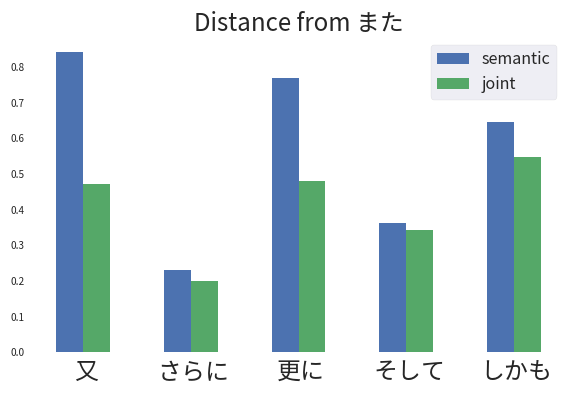
\includegraphics[width=\textwidth]{../images/similarity_ja4.png}
            \caption{Similarity distances between ``また''' (again) and its synonyms are decreasing in the joint embedding}
            \label{fig:similarity_ja4}
        \end{subfigure}
        \caption{The Similarity Distances Between Synonyms in Japanese}
        \label{fig:similarity_ja}
    \end{figure}
    \end{CJK}

\subsection{Homonym and Heteronym} \label{sec:analysis_homonym_heteronym}

We have found positive feedback from tests on both homonyms and heteronyms. The higher correlation between the homonyms vectors indicates that the joint embedding can help the model to improve the noise resistance. The increase in the similarity distance between heteronyms implies that the phonetic information effectively separates them, which is a sign of semantic enhancement.

\begin{figure}[t]
    \centering
    \begin{subfigure}[b]{0.49\textwidth}
        \centering
        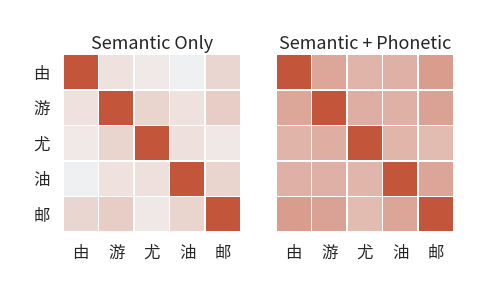
\includegraphics[width=\textwidth]{../images/corr_zh1.png}
        \caption{Pearson correlation between characters spelling \\``ㄧㄡˊ'' (yóu) is increasing in joint embedding}
        \label{fig:corr_zh1}
    \end{subfigure}
    \hfill
    \begin{subfigure}[b]{0.49\textwidth}
        \centering
        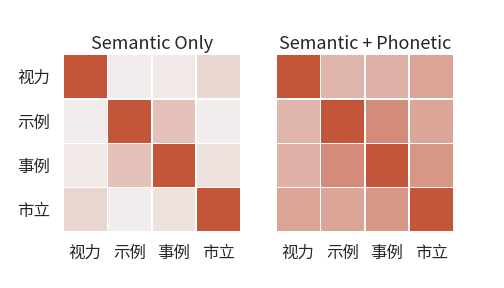
\includegraphics[width=\textwidth]{../images/corr_zh2.png}
        \caption{Pearson correlation between words spelling \\``ㄕˋ ㄌㄧˋ'' (shì lì) is increasing in joint embedding}
        \label{fig:corr_zh2}
    \end{subfigure}
    \begin{subfigure}[b]{0.49\textwidth}
        \centering
        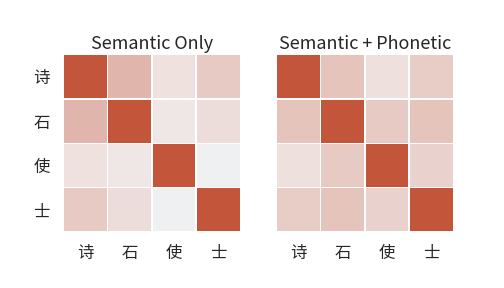
\includegraphics[width=\textwidth]{../images/corr_zh3.png}
        \caption{Pearson correlation between characters spelling ``ㄕ'' (shi) with different tones is increasing in joint embedding}
        \label{fig:corr_zh3}
    \end{subfigure}
    \caption{Pearson Correlation Between Homonyms in Chinese}
    \label{fig:corr_zh}
\end{figure}

\subsubsection{Homonym}

In Figure~\ref{fig:corr_zh}, we examine the correlations between Chinese homonyms in three scenarios. They are the correlation of homophonic characters (Figure~\ref{fig:corr_zh1}), the correlation of homophonic words (Figure~\ref{fig:corr_zh2}), and the correlation of words with identical spelling but different tones (Figure~\ref{fig:corr_zh3}). The results show that the correlation of homonyms is rising for characters, words, and even characters with different tones. 

In Figure~\ref{fig:corr_ja}, we also examine the correlations between Japanese homonyms in three scenarios. Since there are no tones in Japanese, we tested the homonyms with single syllable (Figure~\ref{fig:corr_ja1}), homonyms with two syllables (Figure~\ref{fig:corr_ja2}), and homophonic words (Figure~\ref{fig:corr_ja3}). All the results have shown that joint embedding can effectively improve the correlation between Japanese homonyms and the robustness to noise.

\begin{figure}[t]
    \centering
    \begin{subfigure}[b]{0.49\textwidth}
        \centering
        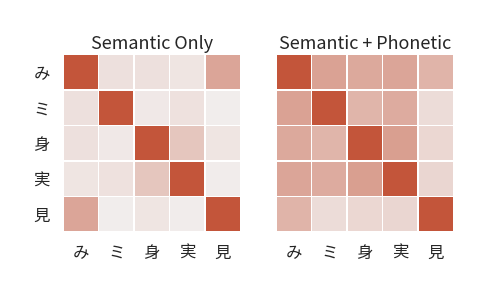
\includegraphics[width=\textwidth]{../images/corr_ja1.png}
        \caption{Pearson correlation between characters with identical spelling (mi) is increasing in joint embedding}
        \label{fig:corr_ja1}
    \end{subfigure}
    \hfill
    \begin{subfigure}[b]{0.49\textwidth}
        \centering
        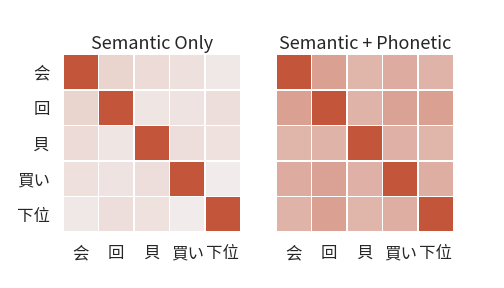
\includegraphics[width=\textwidth]{../images/corr_ja2.png}
        \caption{Pearson correlation between characters and words with identical spelling (kai) is increasing in joint embedding}
        \label{fig:corr_ja2}
    \end{subfigure}
    \begin{subfigure}[b]{0.49\textwidth}
        \centering
        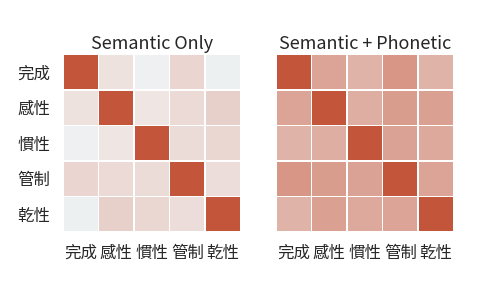
\includegraphics[width=\textwidth]{../images/corr_ja3.png}
        \caption{Pearson correlation between words with identical spelling (kansei) is increasing in joint embedding}
        \label{fig:corr_ja3}
    \end{subfigure}
    \caption{Pearson Correlation between Homonyms in Japanese}
    \label{fig:corr_ja}
\end{figure}

\newpage

\subsubsection{Heteronym}

In Table~\ref{tab:analysis_heteronym1}, we compare the similarity distance between Chinese synonyms. In the first example, ``長'' stands for length (ㄔㄤˊ) and growth (ㄓㄤˇ). In the second example, ``樂'' stands for joyful (ㄌㄜˋ) and harmonious sound (ㄩㄝˋ). In the third example, ``中'' stands for the middle (ㄓㄨㄥ) and suffering (ㄓㄨㄥˋ) respectively. In all three examples, the similarity distances have increased in the joint embedding, which implies that the phonetic information can help distinguish words with the same writing but different spellings and meanings.

\vspace{0.5cm}
\begin{table}[h]
    \centering
        \begin{tabularx}{\textwidth}{bbbb}
            \toprule
            \multirow{2.5}{*}{A} & \multirow{2.5}{*}{B} & \multicolumn{2}{c}{Similarity Distance} \\
            \cmidrule(lr){3-4} {} & {} & Semantic & Joint \\\midrule
            長 (ㄔㄤˊ) 度 & 長 (ㄓㄤˇ) 大 & 0.826 & \textbf{0.853} \\
            樂 (ㄌㄜˋ) 趣 & 音樂 (ㄩㄝˋ) & 0.636 & \textbf{0.682} \\
            中 (ㄓㄨㄥ) 午 & 中 (ㄓㄨㄥˋ) 毒 & 0.842 & \textbf{0.866} \\\bottomrule
        \end{tabularx}
    \caption{Similarity Distance between Heteronyms in Chinese}
    \label{tab:analysis_heteronym1}
\end{table}

\newpage

\begin{CJK}{UTF8}{long}
    In Table~\ref{tab:analysis_heteronym2}, the same advantage also appears in Japanese. We have compared the different spellings and meanings of ``生''. They are raw (なま), life (しょう), birth (う), and crude (き). All the results show that joint embedding can increase the similarity distance between them.
\end{CJK}

\vspace{0.4cm}    
\begin{table}[h]
    \centering
    \begin{CJK}{UTF8}{long}
        \begin{tabularx}{\textwidth}{bbbb}
            \toprule
            \multirow{2.5}{*}{A} & \multirow{2.5}{*}{B} & \multicolumn{2}{c}{Similarity Distance} \\
            \cmidrule(lr){3-4} {} & {} & Semantic & Joint \\\midrule
            生 (なま) & 一生 (しょう) & 0.879 & \textbf{0.889} \\
            生 (なま) & 生 (う) む & 0.830 & \textbf{0.839} \\
            生 (なま) & 生 (き) 地 & 0.769 & \textbf{0.867} \\\bottomrule
        \end{tabularx}
    \end{CJK}
    \caption{Similarity Distance between Heteronyms in Japanese}
    \label{tab:analysis_heteronym2}
\end{table}

\begin{CJK}{UTF8}{long}
    There is a special feature in Japanese where each word usually has more than two different spellings, but the meanings are very similar. These spellings are called 訓読み (Kunyomi) and 音読み (Onyomi). We examine these words in Table~\ref{tab:analysis_heteronym3}. For example, when ``土'' is pronounced as ``つち'' or ``と'', it means soil; when ``海'' is pronounced as ``うみ'' or ``かい'', it means sea; when ``時'' is pronounced as ``とき'' or ``じ'', it means time. The joint embedding is not affected much by heteronyms and correctly reduces the distance of these words; the reason is possibly due to the well-balanced between semantics and phonetics.
\end{CJK}

\vspace{0.4cm}    
\begin{table}[h]
    \centering
    \begin{CJK}{UTF8}{long}
        \begin{tabularx}{\textwidth}{bbbb}
            \toprule
            \multirow{2.5}{*}{A} & \multirow{2.5}{*}{B} & \multicolumn{2}{c}{Similarity Distance} \\
            \cmidrule(lr){3-4} {} & {} & Semantic & Joint \\\midrule
            土 (つち) & 土 (と) 地 & 0.719 & \textbf{0.672} \\
            海 (うみ) & 深海 (かい) & 0.707 & \textbf{0.637} \\
            時 (とき) & 時 (じ) 間 & 0.578 & \textbf{0.498} \\\bottomrule
        \end{tabularx}
    \end{CJK}
    \caption{Similarity Distance between Kunyomi and Onyomi in Japanese}
    \label{tab:analysis_heteronym3}
\end{table}